% ============================================================
% VI. EXPERIMENTS
% ============================================================
\section{Experiments}
\label{sec:experiments}

This section presents an experimental evaluation of the toolchain on the Franka FR3 robot arm.

% ---- A. Research Questions ----
% ---- B. Dataset ----
\subsection{Dataset}

The primary test platform is the Franka FR3 robot arm \cite{franka2020fr3}, consisting of 8 arm links (link0--link7) plus hand and finger links.
The FR3 robot model is bundled with the repository and includes both visual meshes (COLLADA format files representing the true link geometry) and collision meshes (pre-simplified STL files).
We evaluate on the 8 arm links, which contain the richest geometry variation.
Robots with greater mesh complexity or more diverse link shapes (e.g., quadrupeds, mobile manipulators) may exhibit different trade-offs and are left for future work.

% ---- C. Baselines ----
\subsection{Baselines and Configurations}

For each mode, we evaluate the named presets listed in Table~\ref{tab:presets}.

\begin{table}[t]
\centering
\caption{Modes, presets, and key configuration parameters evaluated in the experiments.}
\label{tab:presets}
\begin{tabular}{@{}llccc@{}}
\toprule
Mode & Preset & Sections & Max Capsules & Adaptive \\
\midrule
Convex & default & -- & -- & -- \\
Sphere & single & -- & 1 per link & -- \\
Sphere & default & -- & -- & -- \\
Capsule & single & 2 & 1 per link & No \\
Capsule & default & 4 & 12 per link & No \\
Capsule & high\_detail & 6 & 16 per link & No \\
\bottomrule
\end{tabular}
\end{table}

For capsule ablations, we additionally evaluate:
\begin{itemize}
    \item Fixed vs.\ adaptive circle fitting.
    \item Section count $N$ values of 2, 4, 6, and 8.
    \item Per-link capsule budget $K_{\max}$ values of 1, 4, 8, 12, and 16.
    \item Splitting enabled ($\rho_{\max}=1.45$) vs.\ disabled ($\rho_{\max}=-1$).
    \item Visual mesh vs.\ collision mesh source.
\end{itemize}

% ---- D. Experimental Setup ----
\subsection{Experimental Setup}

All experiments are run on a single machine with an Intel Core i7-13700K CPU, 32~GB RAM, and an NVIDIA RTX 4090 GPU (used only for PyBullet visualization, not for computation).
The pipeline is invoked via Docker, using the Python API with visual mesh source unless otherwise noted.
Runtimes are reported as wall-clock time averaged over three runs and include Docker container startup overhead (approximately 1--2~s per invocation).
The capsule union volume is estimated with $S = 64$ samples per axis (twice the default of $S = 32$) during validation to improve estimate accuracy, while generation uses the default for speed.

% ---- E. Mode Comparison ----
\subsection{Mode Comparison}

Table~\ref{tab:mode_comparison} presents the aggregate results for all six preset-mode combinations on the FR3 arm.
Per-link data and full experiment logs are available in the artifact directory.
Figure~\ref{fig:qualitative_overlay} provides a qualitative visual comparison of the three approximation modes on a representative link (FR3 link3).

\begin{table}[t]
\centering
\caption{Aggregate mode comparison on the Franka FR3 arm (8 links: link0--link7). Worst-case metrics report the maximum (worst) value across all arm links.}
\label{tab:mode_comparison}
\resizebox{\columnwidth}{!}{%
\begin{tabular}{@{}lcrrrr@{}}
\toprule
Mode & Preset & Primitives & Worst $\mathrm{capV/aabb}$ & Worst $r$/binMed & Runtime (s) \\
\midrule
Convex & default & 8 & -- & -- & 0.5 \\
Sphere & single & 8 & -- & -- & 10.1 \\
Sphere & default & 63 & -- & -- & 40.7 \\
Capsule & single & 8 & 1.37 & 1.27 & 12.7 \\
Capsule & default & 10 & 1.47 & 1.50 & 33.0 \\
Capsule & high\_detail & 10 & 1.32 & 1.32 & 21.8 \\
\bottomrule
\multicolumn{6}{@{}l}{\small \textit{Note.} Dash (---) indicates metric not applicable ($\mathrm{capV/aabb}$ and $r$/binMed are capsule-specific).}\\
\end{tabular}%
}
\end{table}

\textbf{Convex mode} produces one convex hull per link (8 primitives) in 0.5~s. Coverage is guaranteed by construction, but the output is mesh-based and lacks closed-form distance evaluation.

\textbf{Sphere-tree modes} trade primitive count against tightness. The \emph{single} preset (8 spheres) achieves near-perfect coverage ($2\times 10^{-5}$~m worst-case gap), while the \emph{default} preset (63 spheres) leaves all links with small uncovered regions (worst $1.8\times 10^{-2}$~m) by design — the medial-axis decomposition fits the shape interior, not the full surface.

\textbf{Capsule modes} produce 8--10 primitives with quantifiable tightness: $\mathrm{capV/aabb}$ ranges from 1.32 to 1.47 and $r$/binMed from 1.27 to 1.50 across presets. The \emph{high\_detail} preset achieves the best worst-case uncovered distance (2.3~mm). Runtime spans 12.7~s (\emph{single}) to 33.0~s (\emph{default}).

\textbf{No analytic-primitive mode achieves complete coverage on all links.} Only convex mesh output guarantees full enclosure; sphere and capsule modes inherently trade coverage for tightness.

\begin{figure}[t]
\centering
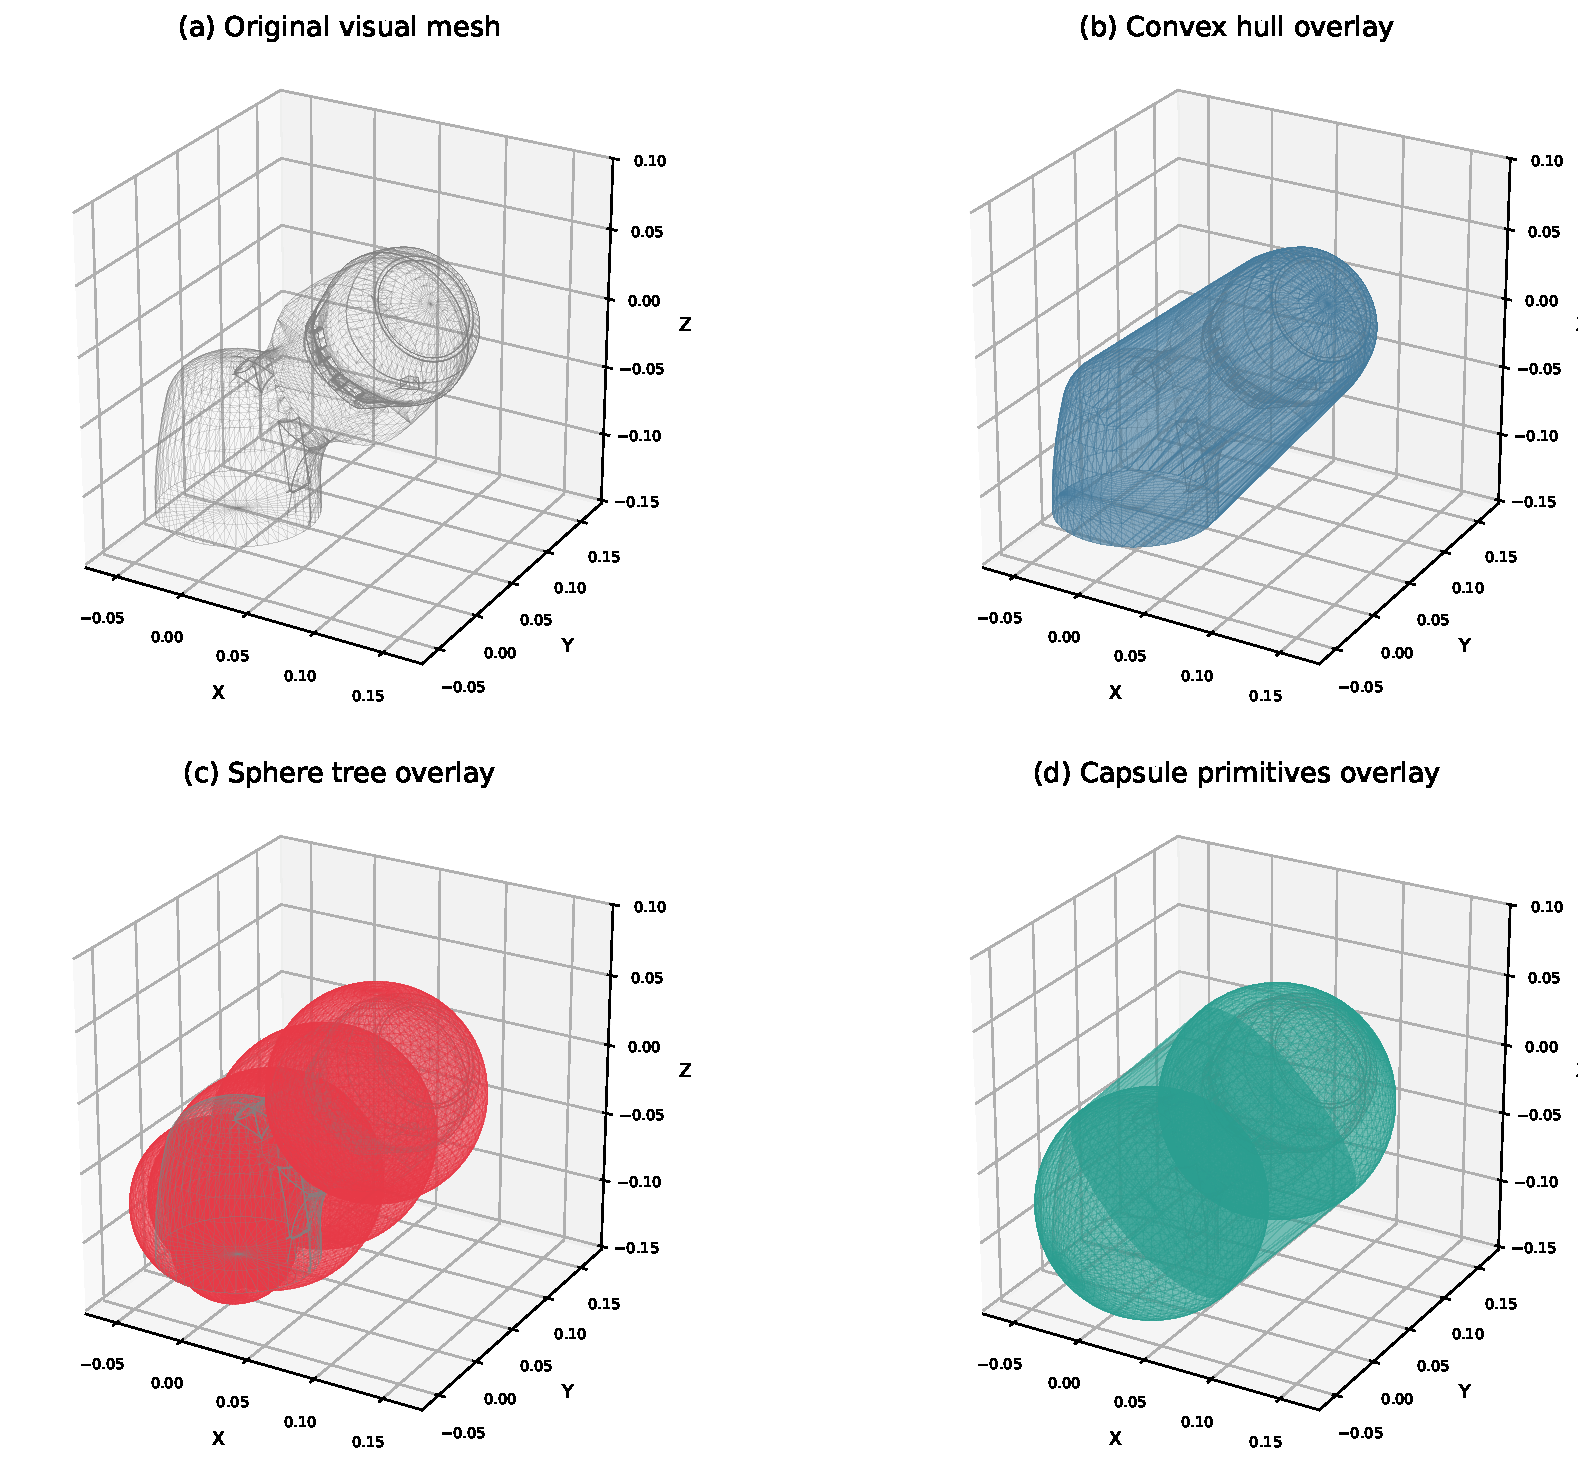
\includegraphics[width=\linewidth]{figures/fig_qualitative_overlay.pdf}
\caption{Qualitative comparison of approximation modes on FR3 link3. The original visual mesh is shown in gray (background); (a) convex hull, (b) sphere tree (default preset), and (c) capsule primitives (default preset) are overlaid as translucent colored geometry. Note: the convex hull overlay is computed via Trimesh as a visual proxy; the production pipeline uses CGAL's Quickhull~\cite{barber1996quickhull} via libigl and may produce a different mesh.}
\label{fig:qualitative_overlay}
\end{figure}

% ---- F. Capsule Ablation ----
\subsection{Capsule Ablation}

Table~\ref{tab:capsule_ablation} reports the effect of individual capsule-fitting parameters.
Each row varies one parameter from the default configuration ($N=4$, $K_{\max}=12$, adaptive circles disabled, $\rho_{\max}=1.45$, visual mesh source) while holding others fixed.

\begin{table}[t]
\centering
\caption{Capsule ablation on the FR3 arm. Each row varies one parameter from the default configuration. Worst-case metrics are across all 8 arm links.}
\label{tab:capsule_ablation}
\resizebox{\columnwidth}{!}{%
\begin{tabular}{@{}lccrrrr@{}}
\toprule
Variant & Change & Caps. & Worst Dist.\ (mm) & $\mathrm{capV/aabb}$ & $r$/binMed & Time (s)\\
\midrule
$N=2$ & Sections reduced & 8 & 6.69 & 1.37 & 1.27 & 13.8 \\
$N=4$ (default) & -- & 10 & 10.23 & 1.47 & 1.50 & 33.0 \\
$N=6$ & Sections increased & 10 & 2.34 & 1.32 & 1.32 & 21.0 \\
$N=8$ & Sections increased & 11 & 1.20 & 1.56 & 1.46 & 21.2 \\
\midrule
$K_{\max}=1$ & Budget reduced & 8 & 10.21 & 1.33 & 1.31 & 14.7 \\
$K_{\max}=4$ & Budget reduced & 10 & 10.23 & 1.47 & 1.50 & 32.6 \\
$K_{\max}=8$ & Budget reduced & 10 & 10.23 & 1.47 & 1.50 & 32.4 \\
$K_{\max}=16$ & Budget increased & 10 & 10.23 & 1.47 & 1.50 & 32.5 \\
\midrule
Adaptive on & $\tau_{\mathrm{coa}}$ active & 39 & 1.35 & 1.41 & 2.05 & 56.8 \\
\midrule
$\rho_{\max}=-1$ & Splitting disabled & 10 & 10.23 & 1.47 & 1.50 & 12.6 \\
\midrule
Collision mesh & Mesh source & 10 & 10.23 & 1.47 & 1.50 & 32.5 \\
\bottomrule
\end{tabular}%
}
\end{table}

\textbf{Section count $N$} is the dominant control parameter. Increasing $N$ from 2 to 8 reduces worst-case uncovered distance from 6.69~mm to 1.20~mm (5.6$\times$ improvement) at the cost of raising capsule count from 8 to 11 and $\mathrm{capV/aabb}$ from 1.37 to 1.56. The relationship is not monotonic: $N=4$ (10.23~mm worst) performs \emph{worse} than $N=2$ (6.69~mm) because the 4-section fit splits one link into two capsules, creating a coverage gap at the boundary. At $N=8$, this gap nearly disappears (to single-digit micrometers).

\textbf{Per-link capsule budget $K_{\max}$} plateaus above 4: all configurations produce identical output (10 capsules, same metrics), indicating that the split-logic threshold $\delta_{\min} = 5 \times 10^{-3}$ rejects additional capsules as not beneficial.

\textbf{Adaptive circle fitting} increases capsule count from 10 to 39 (3.9$\times$) and runtime from 33~s to 57~s. Worst-case uncovered distance improves from 10.23~mm to 1.35~mm (7.6$\times$), but $r$/binMed spikes to 2.05 on one link.

\textbf{Radius-inflation control $\rho_{\max}$} set to --1 (disabling splitting) produces output identical to the default ($\rho_{\max}=1.45$), confirming that COA threshold and $\delta_{\min}$ already prevent excessive radius variation before $\rho_{\max}$ becomes active.

\textbf{Mesh source} (visual vs.\ collision) produces identical capsule fits on the FR3; this may not generalize to robots where collision and visual meshes diverge significantly.

\textbf{No configuration achieves full coverage on all links---every variant leaves at least one link with a positive worst-case signed distance, confirming that the coverage-tightness trade-off is fundamental to the capsule representation.}
